
\documentclass{article}

\usepackage{fancyheadings}
\usepackage{amsmath}
\usepackage{amsfonts}
\usepackage{amssymb}
\usepackage{epsfig}
\usepackage{graphicx}
%\usepackage{doublespace}

\usepackage{KenChuArticleStyle}

%%%%%%%%%%%%%%%%%%%%%%%%%%%%%%%%%%%%%%%%%%%%%%
%%%%%%%%%%%%%%%%%%%%%%%%%%%%%%%%%%%%%%%%%%%%%%
%%%%%%%%%%%%%%%%%%%%%%%%%%%%%%%%%%%%%%%%%%%%%%
%%%%%%%%%%%%%%%%%%%%%%%%%%%%%%%%%%%%%%%%%%%%%%
%%%%%%%%%%%%%%%%%%%%%%%%%%%%%%%%%%%%%%%%%%%%%%

\begin{document}

%%%%%%%%%%%%%%%%%%%%%%%%%%%%%%%%%%%%%%%%%%%%%%

%\setcounter{page}{1}

\pagestyle{fancy}

%\input{../CourseSemesterUnique}

%\rhead[\CourseSemesterUnique]{Kenneth Chu (300517641)}
%\lhead[Kenneth Chu (300517641)]{\CourseSemesterUnique}
\rhead[Study Notes]{Kenneth Chu (300517641)}
\lhead[Kenneth Chu (300517641)]{Study Notes}
\chead[]{{\Large\bf The Student $t$ Distribution} \\
\vskip 0.1cm \normalsize \today}
\lfoot[]{}
\cfoot[]{}
\rfoot[]{\thepage}

%%%%%%%%%%%%%%%%%%%%%%%%%%%%%%%%%%%%%%%%%%%%%%

          %%%%% ~~~~~~~~~~~~~~~~~~~~ %%%%%

\section{Motivation}
\setcounter{theorem}{0}

Let $\left\{\,X_{i} : \Omega\longrightarrow\Re\,\right\}_{i\in\N}$ be a sequence of independent and identically distributed (\emph{i.i.d.}) random variables, with common mean (expected value) $\mu := E\!\left(X_{i}\right)$, for any $i\in\N$, and finite variance $\sigma^{2} > 0$.  For each $n\in\N$, let
\begin{equation*}
\overline{X}_{n} \; := \; \dfrac{1}{n}\,\sum_{i=1}^{n}X_{i}
\quad\quad\textnormal{and}\quad\quad
Z_{n} \; := \; \dfrac{\overline{X}_{n}-\mu}{\sigma/\sqrt{n}}.
\end{equation*}
The random variable $\overline{X}_{n}$ is called the \emph{sample mean} (of the sample consisting of $X_{1}, \ldots, X_{n}$).  Then,
\begin{itemize}
\item  $E\!\left(\overline{X}_{n}\right) = \mu$ and $\Var\!\left(\overline{X}_{n}\right) = \dfrac{\sigma^{2}}{n}$.
          Thus, $\overline{X}_{n}$ is an unbiased estimator for the parameter $\mu$, and
          for large $n$, any observed value of $\overline{X}_{n}$ is expected to closely approximate $\mu$
          (since $\Var\!\left(\overline{X}_{n}\right)\longrightarrow 0$ as $n \longrightarrow \infty$).

          Thus, we may estimate the value of the parameter $\mu$ by taking the average
          $\overline{x} := \dfrac{1}{n}\,\underset{i=1}{\overset{n}{\sum}}x_{i}$ of a set of sampled values
          $x_{1}, \ldots, x_{n}$ of $X_{1}, \ldots, X_{n}$, respectively.
          
\item  Assume the value of $\sigma^{2} > 0$ is known while that of $\mu$ is not known.
          Then, given any explicit candidate value $\mu_{0}$ for the unknown parameter $\mu$,
          we may assess the reliability of the hypothesis $\mu=\mu_{0}$ by taking sampled
          values $x_{1}, \ldots, x_{n}$ for $X_{1}, \ldots, X_{n}$, respectively.

          Given the sampled values $x_{1}, \ldots, x_{n}$, define
          $\overline{x} := \dfrac{1}{n}\,\underset{i=1}{\overset{n}{\sum}}x_{i}$.
          By the Central Limit Theorem, the distribution of $Z_{n}$ approaches
          the standard normal distribution $\mathcal{N}(0,1)$ as $n\longrightarrow\infty$,
          which allows us to approximate the conditional probability
          $P\!\left(\left.\left\vert\overline{X}_{n}-\mu\right\vert\geq\left\vert\overline{x}-\mu\right\vert\;\right\vert\;\mu=\mu_{0}\right)$
          as follows:
          \begin{eqnarray*}
          P\!\left(\left.\left\vert\overline{X}_{n}-\mu\right\vert \geq \left\vert\overline{x}-\mu\right\vert\;\right\vert\;\mu=\mu_{0}\right)
          &=&
          P\!\left(\left.\dfrac{\left\vert\overline{X}_{n}-\mu\right\vert}{\sigma/\sqrt{n}}
                            \geq
                            \dfrac{\left\vert\overline{x}-\mu\right\vert}{\sigma/\sqrt{n}}
          \;\right\vert\;\mu=\mu_{0}\right) \\
          &\approx&
          P\!\left(\left.\left\vert\,Z_{n}\,\right\vert
                            \geq
                            \dfrac{\left\vert\overline{x}-\mu\right\vert}{\sigma/\sqrt{n}}
          \;\right\vert\;\mu=\mu_{0}\right),
          \;\;\textnormal{for large $n$.}
          \end{eqnarray*}
          The conditional probability
          $P\!\left(\left.\left\vert\,Z\,\right\vert\geq\dfrac{\left\vert\overline{x}-\mu\right\vert}{\sigma/\sqrt{n}}\;\right\vert\;\mu=\mu_{0}\right)$ is called the $p$-value corresponding to the set $\{x_{1},\ldots,x_{n}\}$ of sampled values
          under the null hypothesis $\mu = \mu_{0}$.  If the $p$-value subceeds a certain threshold $\alpha$
          (common values for $\alpha$ include $0.05$ and $0.01$), the null hypothesis $\mu=\mu_{0}$ is rejected,
          the underlying intuition being that, under the assumption $\mu=\mu_{0}$, the probability of
          obtaining a set of sampled values ``as extreme as or more extreme than''
          $\{x_{1},\ldots,x_{n}\}$ is ``too low'' (i.e. subceeding $\alpha$).
\end{itemize}
However, the hypothesis test mentioned above relies on the requirement that the value of $\sigma^{2} > 0$ be known.  In practice, this is seldom the case.  In the predominant case that the value of $\sigma^{2}$ is unknown, we could only approximate the value of $\sigma^{2}$ based on sampled data somehow.

To this end, we now assume that $X_{1},X_{2},\ldots\sim \mathcal{N}(\mu,\sigma^{2})$, i.e. the random variables $X_{1},X_{2},\ldots$ are \emph{i.i.d.} normal random variables, where the values of both $\mu$ and $\sigma^{2}$ are not known.  The maximum likelihood estimators for $\mu$ and $\sigma^{2}$, based on sampled values for $X_{1}, \ldots, X_{n}$, are then respectively
\begin{equation*}
\widehat{\mu}_{\textnormal{MLE}} \; = \; \overline{X}_{n} \; := \; \dfrac{1}{n}\sum_{i=1}^{n}X_{i}\,
\quad\quad \textnormal{and} \quad\quad
\widehat{\sigma^{2}}_{\textnormal{MLE}} \; = \; \dfrac{1}{n}\sum_{i=1}^{n}\left(X_{i}-\overline{X}_{n}\right)^{2}.
\end{equation*}
See Example 4, \S8.3, \cite{EwensGrant} for the derivation of $\widehat{\mu}_{\textnormal{MLE}}$ and $\widehat{\sigma^{2}}_{\textnormal{MLE}}$.
Now, $E\!\left(\widehat{\mu}_{\textnormal{MLE}}\right) = E\!\left(\overline{X}_{n}\right) = \mu$; so, $\widehat{\mu}_{\textnormal{MLE}}$ is an unbiased estimator for $\mu$.  On the other hand,
\begin{equation*}
E\!\left(\sum_{i=1}^{n}\left(X_{i}-\overline{X}_{n}\right)^{2}\right) \; = \; (n-1)\,\sigma^{2}.
\end{equation*}
Consequently,
\begin{equation*}
           E\!\left(\widehat{\sigma^{2}}_{\textnormal{MLE}}\right)
\;\;=\;\; E\!\left(\dfrac{1}{n}\sum_{i=1}^{n}\left(X_{i}-\overline{X}_{n}\right)^{2}\right)
\;\;=\;\; \left(\frac{n-1}{n}\right)\sigma^{2}.
\end{equation*}
Thus, $\widehat{\sigma^{2}}_{\textnormal{MLE}}$ is NOT an unbiased estimator for $\sigma^{2}$, but $S_{n}^{2}$ is an unbiased estimator for $\sigma^{2}$, where $S_{n}^{2}$, called the \emph{unbiased sample variance}, is defined by:
\begin{equation*}
S_{n}^{2} \; := \; \dfrac{1}{n-1}\sum_{i=1}^{n}\,\left(X_{i}-\overline{X}_{n}\right)^{2}.
\end{equation*}
Hence, in the case that $X_{1},X_{2},\ldots$ are \emph{i.i.d.} normal random variables with common distribution $\mathcal{N}(\mu,\sigma^{2})$, we may assess the reliability of the hypothesis $\mu = \mu_{0}$, for some candidate value $\mu_{0}$ for the parameter $\mu$, provided we know the probability distribution of \textbf{\emph{Student's $t$ ratio}}, which is defined by:
\begin{equation*}
T_{n-1} \; := \; \dfrac{\overline{X}_{n} - \mu}{\sqrt{S_{n}^{2}\,/\,n}}.
\end{equation*}
The probability distribution of $T_{n-1}$ is the \textbf{\emph{Student $t$ distribution with $(n-1)$ degrees of freedom}}.

          %%%%% ~~~~~~~~~~~~~~~~~~~~ %%%%%

\section{Summary}
\setcounter{theorem}{0}

\begin{itemize}
\item  Let $X_{1}, X_{2}, \ldots, X_{n}$ be \emph{i.i.d.} normal random variables
          with common mean $\mu$ and finite variance $\sigma^{2} > 0$.
          \begin{equation*}
          \overline{X}_{n} \; := \; \dfrac{1}{n}\,\sum_{i=1}^{n}X_{i}\,,
          \quad\quad\textnormal{and}\quad\quad
          S_{n}^{2} \; := \; \dfrac{1}{n-1}\,\sum_{i=1}^{n}\,\left(X_{i}-\overline{X}_{n}\right)^{2}.
          \end{equation*}
          $\overline{X}_{n}$ is called the \textbf{\emph{sample mean}}, and $S_{n}^{2}$ is called the
          (\textbf{\emph{unbiased}}) \textbf{\emph{sample variance}}.
          They are random variables and are unbiased estimators for $\mu$ and $\sigma^{2}$, respectively.
\item  Note that
          \begin{equation*}
          T_{n-1}
          \;\;:=\;\; \dfrac{\overline{X}_{n} - \mu}{\sqrt{S_{n}^{2}\,/\,n}}
          \;\; =\;\; \dfrac{\dfrac{\overline{X}-\mu}{\sigma/\sqrt{n}}}
                      {\sqrt{\left.\left(\dfrac{(n-1)\,S_{n}^{2}}{\sigma^{2}}\right)\right/(n-1)}}.
          \end{equation*}
          We claim:
          \begin{itemize}
          \item  The numerator $\dfrac{\overline{X}_{n}-\mu}{\sigma/\sqrt{n}}$ of $T_{n-1}$
                    has the standard normal distribution.
          \item  The term $\dfrac{(n-1)\,S_{n}^{2}}{\sigma^{2}}$ in the denominator of $T_{n-1}$
                    is a random variable whose distribution is a $\chi^{2}$ distribution
                    with $(n-1)$ degrees of freedom.
          \item  The two random  variables $\dfrac{\overline{X}_{n}-\mu}{\sigma/\sqrt{n}}$ and
                    $\dfrac{(n-1)\,S_{n}^{2}}{\sigma^{2}}$ are independent of each other.
          \end{itemize}
\item  \begin{definition}\mbox{}\\
          Let $Z$ be a standard normal random variable and
          $X$ be a $\chi^{2}$ random variable with $n$ degrees of freedom.
          Suppse $Z$ and $X$ are independent.
          The \textbf{Student $t$ distribution with $n$ degrees of freedom} is the probability distribution of the following
          random variable:
          \begin{equation*}
          T_{n} \; := \; \dfrac{Z}{\sqrt{X/n}}.
          \end{equation*}
          The random variable $T_{n}$ is called the \textbf{Student's $t$ ratio with $n$ degrees of freedom}.
          \end{definition}
\item  \begin{theorem}\mbox{}\\
          The probability density function of the Student $t$ distribution with $n$ degrees of freedom is given by:
          \begin{equation*}
          f_{T_{n}}(t) \; = \; \dfrac{\Gamma\!\left(\dfrac{n+1}{2}\right)}{\sqrt{n\,\pi}\,\Gamma\!\left(\dfrac{n}{2}\right)}
                                      \cdot
                                      \dfrac{1}{\left(1+\dfrac{t^{2}}{n}\right)^{(n+1)/2}}\,,
          \quad\textnormal{for}\;\; -\infty < t < \infty.
          \end{equation*}
          \end{theorem}
\end{itemize}

The diagram below shows the graphs of the probability density functions $f_{T_{20}}$ in black and $f_{T_{2}}$ in red.
\begin{center}
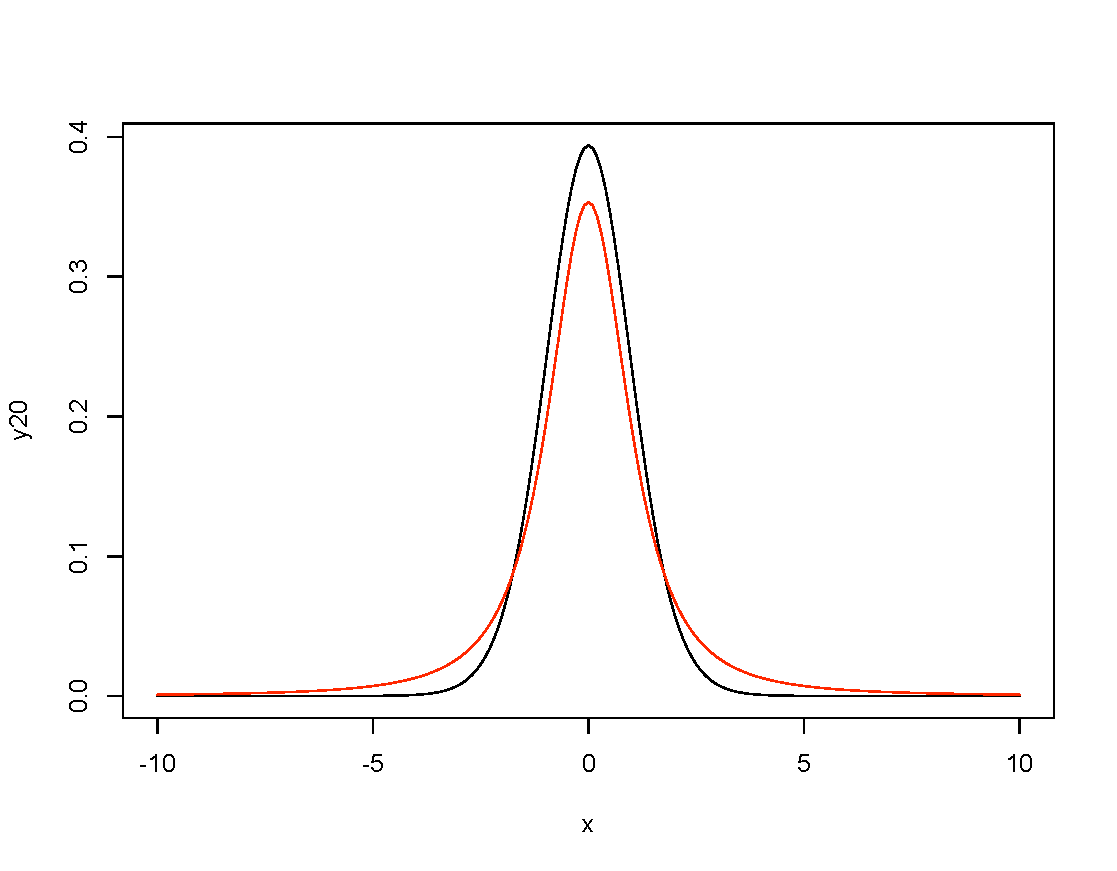
\includegraphics[height=10.0cm,width=16cm]{StudentTDist-df20-df2.pdf}
\end{center}
The above graph is generated with \texttt{R} with the following command:
\begin{center}
\texttt{> y20 = dt(x,df=20); y2 = dt(x,df=2); plot(x,y20,type="l"); points(x,y2,type="l",col="red");}
\end{center}

          %%%%% ~~~~~~~~~~~~~~~~~~~~ %%%%%

\section{$\chi^{2}_{n}$ --- the distribution of the sum of squares of $n\in\N$ independent standard normal random variables}
\setcounter{theorem}{0}

\begin{theorem}\mbox{}\\
Let $Z_{1}, Z_{2}, \ldots, Z_{n}$ be $n$ independent standard normal random variables, and let
$X := \underset{i=1}{\overset{n}{\sum}}\,Z_{i}^{2}$.
Then, $X$ has a Gamma distribution with parameter values $r = \dfrac{n}{2}$ and $\lambda = \dfrac{1}{2}$.
Equivalently, the probability density function of $X$ is given by
\begin{equation*}
f_{X}(x) \; = \; \dfrac{1}{2^{n/2}\,\Gamma\!\left(\dfrac{n}{2}\right)} \; x^{(n/2)-1} \; e^{-x/2}\,,
\quad\textnormal{for}\;\; x \geq 0.
\end{equation*}
\end{theorem}
\proof
First, take $m=1$.  We claim that $Z^{2} \sim \Gamma(r,\lambda)$, for $r = \lambda =\dfrac{1}{2}$,
where $\Gamma(r,\lambda)$ denotes the Gamma distribution.
Indeed, for any $x \geq 0$,
\begin{eqnarray*}
            F_{Z^{2}}(x)
& = &   P\!\left(Z^{2}\leq x\right)
\;\;=\;\;  P\!\left(-\sqrt{x} \leq Z \leq\sqrt{x}\right)
\;\;=\;\; 2\,P\!\left(0 \leq Z \leq\sqrt{x}\right) \\
& = &   2 \, \int_{0}^{\sqrt{x}}f_{Z}(\zeta)\,\d\zeta
\;\;=\;\; 2 \, \int_{0}^{\sqrt{x}}\dfrac{1}{\sqrt{2\,\pi}}\,e^{-\zeta^{2}/2}\,\d\zeta \\
& = &  \sqrt{\dfrac{2}{\pi}} \int_{0}^{\sqrt{x}}e^{-\zeta^{2}/2}\,\d\zeta.
\end{eqnarray*}
Differentiating $F_{Z^{2}}(x)$ with respect to $x$ yields:
\begin{eqnarray*}
       f_{Z^{2}}(x)
&=& \dfrac{\d}{\d x}\,F_{Z^{2}}(x)
\;=\; \sqrt{\dfrac{2}{\pi}}\,\dfrac{\d}{\d x}\!\left(\int_{0}^{\sqrt{x}}e^{-\zeta^{2}/2}\,\d\zeta\right)
\;=\; \sqrt{\dfrac{2}{\pi}}\,e^{-x/2}\,\dfrac{\d}{\d x}\!\left(\sqrt{x}\right)
\;=\; \sqrt{\dfrac{2}{\pi}}\,e^{-x/2}\,\dfrac{1}{2\,\sqrt{x}} \\
&=& \dfrac{1}{\sqrt{2}\;\Gamma\!\left(\frac{1}{2}\right)}\;x^{(1/2)-1}\,e^{-x/2},
       \quad\textnormal{for}\;\; x > 0.
\end{eqnarray*}
We have used the fact that $\Gamma\!\left(\frac{1}{2}\right) = \sqrt{\pi}$.
Thus, $f_{Z^{2}}(x)$ is the probability density function of the Gamma distribution $\Gamma(r,\lambda)$ with $r = \dfrac{1}{2}$ and $\lambda=\dfrac{1}{2}$, since for any $r, \lambda > 0$,
\begin{equation*}
f_{\Gamma(r,\lambda)}(y) \; = \; \dfrac{\lambda^{r}}{\Gamma\!\left(r\right)} \; y^{r-1} \; e^{-\lambda y},
\quad\textnormal{for}\;\; y \geq 0.
\end{equation*}
Next, recall that: If $G_{1} \sim \Gamma(r_{1},\lambda)$ and $G_{2} \sim \Gamma(r_{2},\lambda)$ are independent random variables, then $G_{1} + G_{2} \sim \Gamma(r_{1}+r_{2},\lambda)$.  Induction thus immediately gives:  If $G_{i} \sim \Gamma(r_{i},\lambda)$, $i = 1, \ldots, n$, are independent random variables, then
\begin{equation*}
\overset{n}{\underset{i=1}{\sum}}\,G_{i} \;\; \sim \;\; \Gamma\!\left(\sum_{i=1}^{n}r_{i}\,,\,\lambda\right).
\end{equation*}
(See, for example, Theorem 4.6.4, \cite{LarsenMarx}, or \S2.4, \cite{Wasserman2004}).

\noindent
Since $Z_{1}^{2}, Z_{2}^{2}, \ldots, Z_{n}^{2} \sim \Gamma\!\left(r=\frac{1}{2},\lambda=\frac{1}{2}\right)$ and they are independent random variables, it now follows that
\begin{equation*}
X \;\; := \;\; \sum_{i=1}^{n} Z_{i}^{2} \;\; \sim \;\; \Gamma\!\left(r=\frac{n}{2}\,,\,\lambda=\frac{1}{2}\right).
\end{equation*}
In other words, the probability density function of $X$ is given by:
\begin{equation*}
         f_{X}(x) \; = \; f_{\Gamma(r=n/2,\lambda=1/2)}(x)
\; = \; \dfrac{\left(\frac{1}{2}\right)^{n/2}}{\Gamma\!\left(\frac{n}{2}\right)} \; x^{(n/2)-1} \; e^{-(1/2)\cdot x}
\; = \; \dfrac{1}{2^{n/2}\,\Gamma\!\left(\dfrac{n}{2}\right)} \; x^{(n/2)-1} \; e^{-x/2}\,,
\quad\textnormal{for}\;\; x > 0,
\end{equation*}
as required.  \qed

\begin{definition}\mbox{}\\
The \textbf{chi-square distribution with $n \in \N$ degree(s) of freedom} is, by definition,
Gamma distribution $\Gamma\!\left(r=\frac{n}{2},\lambda=\frac{1}{2}\right)$.
It is denoted by $\chi^{2}_{n}$.
\end{definition}

\begin{remark}\mbox{}\\
The sum $X := Z_{1}^{2} + Z_{2}^{2} + \cdots + Z_{n}^{2}$ of the squares of $n \in \N$ independent standard normal random variables $Z_{1}, Z_{2}, \ldots, Z_{n} \sim \mathcal{N}(0,1)$ has a chi-square distribution with $n$ degree(s) of freedom.  In other words,
$X := Z_{1}^{2} + Z_{2}^{2} + \cdots + Z_{n}^{2} \sim \chi^{2}_{n}$.
\end{remark}

\begin{remark}\mbox{}\\
Note that
\begin{equation*}
          f_{\chi^{2}_{1}}(x)
\; = \; \dfrac{1}{2^{1/2}\,\Gamma\!\left(\dfrac{1}{2}\right)} \; x^{(1/2)-1} \; e^{-x/2}
\; = \; \dfrac{1}{\sqrt{2}\,\sqrt{\pi}}\;\,x^{-1/2} \; e^{-x/2}
\; = \; \dfrac{1}{\sqrt{2\pi} \cdot x^{1/2} \cdot e^{x/2}}
\end{equation*}
has a singularity at $x=0$, and
\begin{equation*}
          f_{\chi^{2}_{2}}(x)
\; = \; \dfrac{1}{2^{2/2}\,\Gamma\!\left(\dfrac{2}{2}\right)} \; x^{(2/2)-1} \; e^{-x/2}
\; = \; \dfrac{1}{{2}\;\Gamma\!\left(1\right)}\;x^{0} \; e^{-x/2}
\; = \; \dfrac{1}{2}\,e^{-x/2}
\end{equation*}
is simply an exponential decay in $x \geq 0$.
\end{remark}

The diagram below shows graphs of the probability density functions $f_{\chi^{2}_{1}}, \ldots, f_{\chi^{2}_{5}}$.
It is generated with \texttt{R} with the following command:
\vskip 0.2cm
\texttt{
\small
\noindent\mbox{}\\
> x<-seq(0,10,0.001);  \\
> y1<-dchisq(x,df=1); y2<-dchisq(x,df=2); y3<-dchisq(x,df=3); y4<-dchisq(x,df=4); y5<-dchisq(x,df=5); \\
> plot(x,y1,ylim=c(0,0.6),type="l");
> points(x,y2,type="l",col="blue"); points(x,y3,type="l",col="green"); \\
> points(x,y4,type="l",col="red");points(x,y5,type="l",col="cyan"); \\
> legend("topright",c("df=1","df=2","df=3","df=4","df=5"),text.col=c("black","blue","green","red","cyan"));}
\mbox{}
\begin{center}
\vskip -1.3cm
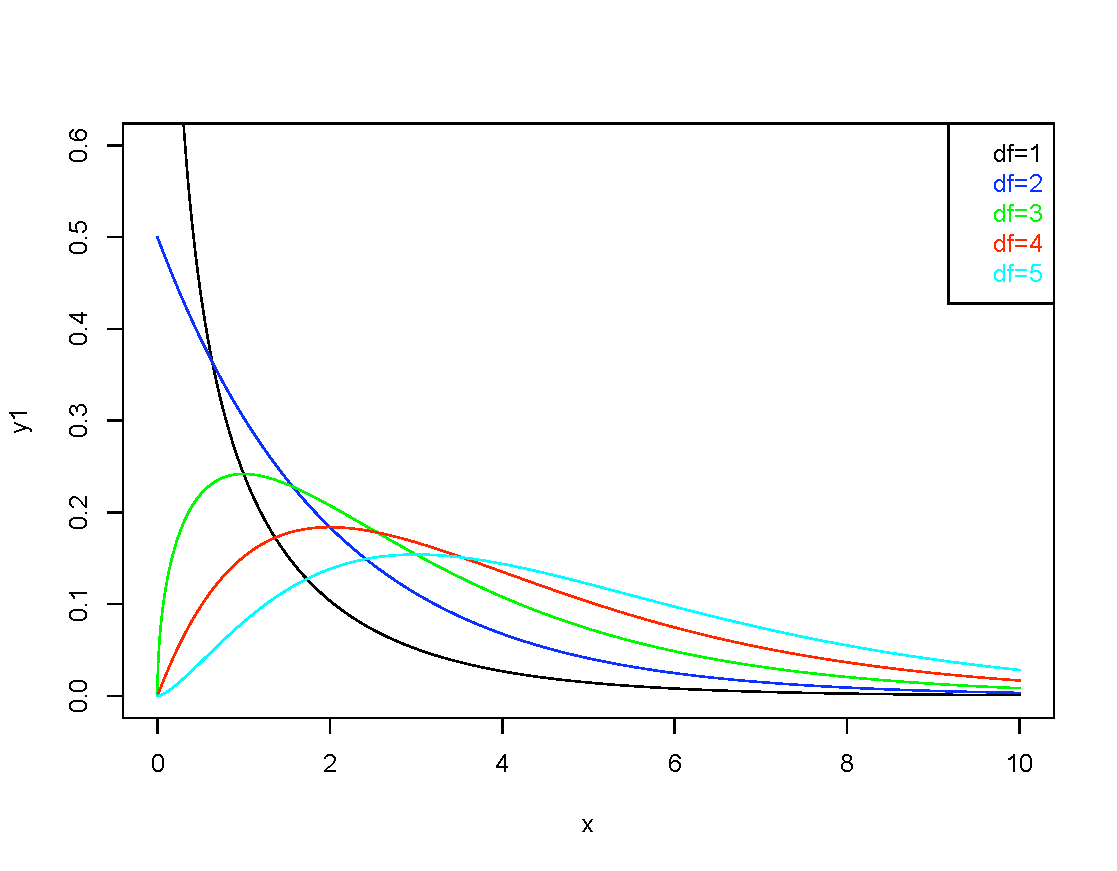
\includegraphics[height=13.0cm,width=16cm]{ChiSquare-df1-thru-df5.pdf}
\end{center}

          %%%%% ~~~~~~~~~~~~~~~~~~~~ %%%%%

\section{$\mathcal{F}^{m}_{n}$ --- the distribution of the ratio of two $\chi^{2}$ random variables}
\setcounter{theorem}{0}

\begin{definition}\mbox{}\\
Let $m,n \in \N$.  Let $X_{m} \sim \chi^{2}_{m}$ and $X_{n} \sim \chi^{2}_{n}$ be independent $\chi^{2}$ random variables with the indicated degrees of freedom.  For $m, n \in \N$, the \textbf{F distribution with $m$ and $n$ degrees of freedom}, denoted by $\mathcal{F}^{m}_{n}$, is the probability distribution of the following random variable:
\begin{equation*}
F := \dfrac{X_{m}/m}{X_{n}/n}.
\end{equation*}
\end{definition}

\begin{theorem}\label{pdf:Fmn}\mbox{}\\
The probability density function of the F distribution $\mathcal{F}^{m}_{n}$ with $m$ and $n$ degrees of freedom is given by:
\begin{equation*}
         f_{\mathcal{F}^{m}_{n}}\!\left(\zeta\right)
\; = \; \left(
         m^{m/2} \cdot n^{n/2}\cdot
         \dfrac{\Gamma\!\left(\frac{m+n}{2}\right)}{\Gamma\!\left(\frac{m}{2}\right)\,\Gamma\!\left(\frac{n}{2}\right)}
         \right)\cdot
         \dfrac{\zeta^{(m/2)-1}}{(m\,\zeta + n)^{(m+n)/2}},
\quad\textnormal{for}\;\; \zeta \geq 0.
\end{equation*}
\end{theorem}

\begin{remark}\mbox{}\\
The ``F'' in ``F distribution'' commemorates the renowned statistician Sir Ronald Fisher. \vskip 0.1cm

\noindent
Let $T = \dfrac{Z}{\sqrt{X/n}}$ be a Student $t$ ratio, i.e. $Z$ and $X$ are independent random variables with $Z \sim \mathcal{N}(0,1)$ and $X \sim \chi^{2}_{n}$.  Then, $Z^{2} \sim \chi^{2}_{1}$.  Hence, $T^{2} = \dfrac{Z^{2}}{X/n} = \dfrac{Z^{2}/1}{X/n} \sim \mathcal{F}^{1}_{n}$, the F distribution with $m=1$ and $n$ degrees of freedom.  We will derive the probability density function for the distribution of $T$ by using that of $T^{2}$ as given by Theorem \ref{pdf:Fmn}.
\end{remark}

\proofof Theorem \ref{pdf:Fmn}:\quad  We first find the probability density function for $X_{m}/X_{n}$.  Now,
\begin{eqnarray*}
                              X_{m} \sim \chi^{2}_{m}
&\Longrightarrow& f_{X_{m}}(x) = \dfrac{1}{2^{m/2}\,\Gamma\!\left(\dfrac{m}{2}\right)} \; x^{(m/2)-1} \; e^{-x/2}, \\
                              X_{n} \sim \chi^{2}_{m}
&\Longrightarrow& f_{X_{n}}(x) = \dfrac{1}{2^{n/2}\,\Gamma\!\left(\dfrac{n}{2}\right)} \; x^{(n/2)-1} \; e^{-x/2}
\end{eqnarray*}
By Theorem \ref{pdf:quotient},
\begin{eqnarray*}
        f_{X_{m}/X_{n}}(x)
&=&  \int_{0}^{\infty}\; |\zeta| \cdot f_{X_{n}}(x) \cdot f_{X_{m}}(x\,\zeta)\;\d\zeta \\
&=&  \int_{0}^{\infty}\;
        \zeta \cdot
        \left(\dfrac{1}{2^{n/2}\,\Gamma\!\left(\dfrac{n}{2}\right)} \; \zeta^{(n/2)-1} \; e^{-\zeta/2}\right) \cdot
        \left(\dfrac{1}{2^{m/2}\,\Gamma\!\left(\dfrac{m}{2}\right)} \; (x\,\zeta)^{(m/2)-1} \; e^{-(x\,\zeta)/2}\right)
        \;\d\zeta \\
&=&  \dfrac{1}{2^{(m+n)/2}\cdot\Gamma\!\left(\dfrac{n}{2}\right)\cdot\Gamma\!\left(\dfrac{m}{2}\right)} \cdot
        \left(x^{(m/2)-1}\right) \cdot
        \left(\int_{0}^{\infty}\;
        \zeta^{\frac{m+n}{2}-1}\cdot \exp\!\left(-\,\frac{1+x}{2}\cdot\zeta\right)
        %\zeta \cdot
        %\left(\zeta^{(n/2)-1} \; e^{-\zeta/2}\right) \cdot
        %\left((x\,\zeta)^{(m/2)-1} \; e^{-(x\,\zeta)/2}\right)\;
        \;\d\zeta\right) \\
\end{eqnarray*}
Now, recall again that the probability density function of the $\Gamma(r,\lambda)$ distribution is given by:
\begin{equation*}
f_{\Gamma(r,\lambda)}(\zeta) \; = \; \dfrac{\lambda^{r}}{\Gamma\!\left(r\right)} \; \zeta^{r-1} \; e^{-\lambda \zeta},
\quad\textnormal{for}\;\; \zeta \geq 0.
\end{equation*}
In particular,
\begin{equation*}
1 \; = \; \int_{0}^{\infty}f_{\Gamma(r,\lambda)}(\zeta)\,\d\zeta \; = \; \int_{0}^{\infty}\dfrac{\lambda^{r}}{\Gamma\!\left(r\right)} \; \zeta^{r-1} \; e^{-\lambda \zeta}\,\d\zeta,
\quad\textnormal{which implies}\quad
\int_{0}^{\infty}\zeta^{r-1} \; e^{-\lambda \zeta}\,\d\zeta
\; = \;
\dfrac{\Gamma\!\left(r\right)}{\lambda^{r}}.
\end{equation*}
We now see that
\begin{eqnarray*}
f_{X_{m}/X_{n}}(x)
&=&
\dfrac{1}{2^{(m+n)/2}\cdot\Gamma\!\left(\frac{n}{2}\right)\cdot\Gamma\!\left(\frac{m}{2}\right)} \cdot
\left(x^{(m/2)-1}\right) \cdot
\left(\int_{0}^{\infty}\;
\zeta^{\frac{m+n}{2}-1}\cdot \exp\!\left(-\,\frac{1+x}{2}\cdot\zeta\right)
\;\d\zeta\right) \\
&=&
\dfrac{1}{2^{(m+n)/2}\cdot\Gamma\!\left(\frac{n}{2}\right)\cdot\Gamma\!\left(\frac{m}{2}\right)} \cdot
\left(x^{(m/2)-1}\right) \cdot
\dfrac{\Gamma\!\left(\frac{m+n}{2}\right)}{\left(\frac{1+x}{2}\right)^{(m+n)/2}} \\
&=&
\dfrac{\Gamma\!\left(\frac{m+n}{2}\right)}{\Gamma\!\left(\frac{m}{2}\right)\cdot\Gamma\!\left(\frac{n}{2}\right)}
\cdot
\dfrac{x^{(m/2)-1}}{\left(1+x\right)^{(m+n)/2}} \\
\end{eqnarray*}
Lastly, note that for any $\alpha > 0$ and random variable $Y$, we have:
\begin{equation*}
       F_{\alpha Y}(y)
\;=\; P\!\left(\alpha Y\leq y\right)
\;=\; P\!\left(Y\leq\frac{1}{\alpha}\,y\right)
\;=\; F_{Y}\!\left(\frac{1}{\alpha}\,y\right).
\end{equation*}
Hence,
\begin{equation*}
       f_{\alpha Y}(y)
\;=\; \dfrac{\d}{\d y}\,F_{\alpha\,Y}(y)
\;=\; \dfrac{\d}{\d y}\,F_{Y}\!\left(\frac{1}{\alpha}\,y\right)
\;=\; F'_{Y}\!\left(\frac{1}{\alpha}\,y\right)\cdot\dfrac{\d}{\d y}\left(\frac{1}{\alpha}\,y\right)
\;=\; \frac{1}{\alpha}\,f_{Y}\!\left(\frac{1}{\alpha}\,y\right).
\end{equation*}
Consequently,
\begin{eqnarray*}
            f_{\frac{X_{m}/m}{X_{n}/n}}(x)
&=&     f_{\left(\frac{n}{m}\right)X_{m}/X_{n}}(x)
\;\;=\;\; \frac{m}{n}\cdot f_{X_{m}/X_{n}}\!\left(\frac{m}{n}\,x\right) \\
&=&     \dfrac{m}{n}\cdot
            \dfrac{\Gamma\!\left(\frac{m+n}{2}\right)}{\Gamma\!\left(\frac{m}{2}\right)\cdot\Gamma\!\left(\frac{n}{2}\right)}
            \cdot
            \dfrac{\left(\frac{m}{n} x\right)^{(m/2)-1}}{\left(1+\frac{m}{n} x\right)^{(m+n)/2}} \\
&=&     \dfrac{m}{n}\cdot\left(\frac{m}{n}\right)^{(m/2)-1}\cdot n^{(m+n)/2}\cdot
            \dfrac{\Gamma\!\left(\frac{m+n}{2}\right)}{\Gamma\!\left(\frac{m}{2}\right)\cdot\Gamma\!\left(\frac{n}{2}\right)}
            \cdot
            \dfrac{x^{(m/2)-1}}{\left(n+mx\right)^{(m+n)/2}} \\
&=&     \left(
           m^{m/2} \cdot n^{n/2} \cdot
           \dfrac{\Gamma\!\left(\frac{m+n}{2}\right)}{\Gamma\!\left(\frac{m}{2}\right)\cdot\Gamma\!\left(\frac{n}{2}\right)}
           \right)
           \cdot
           \dfrac{x^{(m/2)-1}}{\left(mx+n\right)^{(m+n)/2}} \\
\end{eqnarray*}
This completes the proof of Theorem \ref{pdf:Fmn}.  \qed

          %%%%% ~~~~~~~~~~~~~~~~~~~~ %%%%%

\section{The Student $t$ distribution with $n\in\N$ degrees of freedom}
\setcounter{theorem}{0}

\begin{definition}\mbox{}\\
The \textbf{Student $t$ distribution with $n\in\N$ degrees of freedom} is the probability distribution of a random variable $T_{n}$ of the form
\begin{equation*}
T_{n} \; = \; \dfrac{Z}{\sqrt{\dfrac{X}{n}}},
\end{equation*}
where $Z$ and $X$ are independent random variables, $Z$ is a standard normal random variable, and $X$ is a chi-square random variable with $n\in\N$ degrees of freedom.
\end{definition}

\begin{lemma}\mbox{}\\
The probability density function $f_{T_{n}}$ of the Student $t$ distribution is an even function, i.e. $f_{T_{n}}(-t) = f_{T_{n}}(t)$, for any $t \in \Re$.
\end{lemma}

\proof By definition of the Student $t$ distribution, $T_{n} = \dfrac{Z}{\sqrt{X/n}}$, where $Z \sim \mathcal{N}(0,1)$ and $X \sim \chi^{2}_{n}$ are independent random variables.  Consequently, $-T_{n} = \dfrac{-Z}{\sqrt{X/n}}$ also has the Student $t$ distribution, and thus $f_{(-T_{n})}(t) = f_{T_{n}}(t)$ for all $t \in \Re$.  On the other hand,
\begin{equation*}
            F_{(-T_{n})}(t)
\;\;=\;\;  P(-T_{n}\leq t)
\;\;=\;\;  P(T_{n}\geq -t)
\;\;=\;\;  1 - P(T_{n} \leq -t)
\end{equation*}
Differentiating with respect to $t$ yields:
\begin{eqnarray*}
            f_{(-T_{n})}(t)
& = &   \dfrac{\d}{\d t} F_{(-T_{n})}(t)
\;\;=\;\;  \dfrac{\d}{\d t}\!\left(1 - P(T_{n} \leq -t)\right)
\;\;=\;\;  -\dfrac{\d}{\d t} P(T_{n} \leq -t)
\;\;=\;\;  -\left(\dfrac{\d}{\d(-t)} P(T_{n} \leq -t)\right)\cdot\dfrac{\d(-t)}{\d t} \\
& = &   -\, f_{T_{n}}(-t)\,\dfrac{\d(-t)}{\d t}
\;\;=\;\;  f_{T_{n}}(-t).
\end{eqnarray*}
Thus, we have shown:
\begin{equation*}
f_{T_{n}}(-t) \;\; = \;\; f_{(-T_{n})}(t) \;\; = \;\; f_{T_{n}}(t).
\end{equation*}
\qed


\begin{theorem}\label{pdf:StudentT}\mbox{}\\
The probability density function of a random variable $T_{n}$ having the Student $t$ distribution with $n \in \N$ degrees of freedom is given by:
\begin{equation*}
f_{T_{n}}(t) \;\; = \;\;
\left(
\dfrac{1}{\sqrt{n\pi}}\cdot\dfrac{\Gamma\!\left(\frac{n+1}{2}\right)}{\Gamma\!\left(\frac{n}{2}\right)}
\right)
\cdot
\dfrac{1}{\left(1+\dfrac{t^{2}}{n}\right)^{(n+1)/2}}\,,
\quad\textnormal{for}\;\; -\infty < t < \infty\,.
\end{equation*}
\end{theorem}

\proof Note that $T_{n}^{2} = \dfrac{Z^{2}}{X/n} = \dfrac{Z^{2}/1}{X/n} \sim F^{1}_{n}$.  Hence,
\begin{equation*}
f_{T^{2}_{n}}(t) \;=\; \dfrac{n^{n/2}\,\Gamma\!\left(\frac{n+1}{2}\right)}{\Gamma\!\left(\frac{1}{2}\right)\,\Gamma\!\left(\frac{n}{2}\right)}\; t^{-1/2} \; \dfrac{1}{(t+n)^{(n+1)/2}}\,,
\quad\textnormal{for}\;\; t > 0.
\end{equation*}

Since $f_{T_{n}}(t)$ is an even function, we have, for $t  > 0$, 
\begin{eqnarray*}
            F_{T_{n}}(t)
& = &   P(T_{n}\leq t)
\;\;=\;\; \dfrac{1}{2} + P(0\leq T_{n} \leq t)
\;\;=\;\; \dfrac{1}{2} + \dfrac{1}{2}P(-t \leq T_{n} \leq t)
\;\;=\;\; \dfrac{1}{2} + \dfrac{1}{2}P\!\left(0 \leq T_{n}^{2} \leq t\right) \\
& = &   \dfrac{1}{2} + \dfrac{1}{2}F_{T_{n}^{2}}\!\left(t^{2}\right)
\end{eqnarray*}
Differentiating with respect to $t$ yields:
\begin{eqnarray*}
           f_{T_{n}}(t)
& = &   \dfrac{\d}{\d t}F_{T_{n}}(t)
\;\;=\;\; \dfrac{1}{2}F'_{T_{n}^{2}}\!\left(t^{2}\right) \dfrac{\d}{\d t}\!\left(t^{2}\right)
\;\;=\;\; t \cdot f_{T_{n}^{2}}\!\left(t^{2}\right) 
\;\;=\;\; t \cdot
          \dfrac{n^{n/2}\,\Gamma\!\left(\frac{n+1}{2}\right)}{\Gamma\!\left(\frac{1}{2}\right)\,\Gamma\!\left(\frac{n}{2}\right)}
          \cdot \left(t^{2}\right)^{-1/2} \cdot \dfrac{1}{(t^{2}+n)^{(n+1)/2}} \\
& = &  \dfrac{n^{n/2}\,\Gamma\!\left(\frac{n+1}{2}\right)}{\Gamma\!\left(\frac{1}{2}\right)\,\Gamma\!\left(\frac{n}{2}\right)}
           \cdot
           \dfrac{1}{n^{(n+1)/2}\left(1+\dfrac{t^{2}}{n}\right)^{(n+1)/2}} 
\;\;=\;\; \left(
           \dfrac{1}{\sqrt{n\,\pi}}
           \cdot\dfrac{\Gamma\!\left(\frac{n+1}{2}\right)}{\Gamma\!\left(\frac{n}{2}\right)}
           \right)
           \cdot
           \dfrac{1}{\left(1+\dfrac{t^{2}}{n}\right)^{(n+1)/2}}
\end{eqnarray*}
This completes the proof of Theorem \ref{pdf:StudentT}
\qed

%%%%%%%%%%%%%%%%%%%%%%%%%%%%%%%%%%%%%%%%%%%%%%

\appendix

          %%%%% ~~~~~~~~~~~~~~~~~~~~ %%%%%

\section{The Probability Density Function of the Quotient of Two Random Variables}
\setcounter{theorem}{0}

\begin{theorem}\label{pdf:quotient}\mbox{}\\
A
\end{theorem}

          %%%%% ~~~~~~~~~~~~~~~~~~~~ %%%%%

\section{A Technical Result}
\setcounter{theorem}{0}

\begin{theorem}\label{SampleMean:SampleVariance:Independence}\mbox{}\\
Let $X_{1}, X_{2}, \ldots, X_{n}$ be independent standard normal random variables with common mean $\mu$ and (finite) variance $\sigma^{2} > 0 $.  Define:
\begin{equation*}
\overline{X} \; := \; \dfrac{1}{n}\sum_{i=1}^{n}X_{i}
\quad\quad\textnormal{and}\quad\quad
S^{2} \; := \; \dfrac{1}{n-1}\sum_{i=1}^{n}\left(\,X_{i}-\overline{X}\,\right)^{2}\,.
\end{equation*}
Then,
\begin{itemize}
\item  $\overline{X}$ and $S^{2}$ are independent random variables.
\item  $\dfrac{n-1}{\sigma^{2}}\,S^{2}$ has a chi-square distribution with $(n-1)$ degrees of freedom.
\end{itemize}
\end{theorem}

\proof  Let $Y_{i} := \dfrac{X_{i}-\mu}{\sigma}$, $i = 1, \ldots n$.  Then, $Y_{1}, Y_{2}, \ldots, Y_{n} \sim \mathcal{N}(0,1)$, and they are independent random variables.   Let $A \in \Re^{n \times n}$ be any orientation-preserving orthogonal matrix (hence, $A^{T}\cdot A = I_{n \times n}$ and $\det(A) = 1$) whose $n^{\textnormal{th}}$ row is $\left(\frac{1}{\sqrt{n}},\frac{1}{\sqrt{n}},\ldots,\frac{1}{\sqrt{n}}\right)$.  Let $\mathbf{Y}$ be the $\Re^{n}$-valued random variable defined by $\mathbf{Y} := (Y_{1},Y_{2},\ldots,Y_{n})^{T}$, and let $\mathbf{Z}$ be the $\Re^{n}$-valued random variable defined by $\mathbf{Z} := A\cdot\mathbf{Y}$.  Let $Z_{1}, Z_{2}, \ldots, Z_{n}$ denote the component random variables of $\mathbf{Z}$, i.e. $\mathbf{Z} = \left(Z_{1},Z_{2},\ldots,Z_{n}\right)^{T}$.  Note that $Z_{n} = \frac{1}{\sqrt{n}}Y_{1} + \frac{1}{\sqrt{n}}Y_{2} + \cdots + \frac{1}{\sqrt{n}}Y_{n} = \sqrt{n}\,\overline{Y}$, where $\overline{Y} := \frac{1}{n}\sum_{i=1}^{n}Y_{i}$.

For any measurable $\Omega \subset \Re^{n}$,
\begin{eqnarray*}
          P\!\left(\mathbf{Z}\in\Omega\right)
& = & P\!\left(A\cdot\mathbf{Y}\in\Omega\right) \;\; = \;\; P\!\left(\mathbf{Y}\in A^{-1}\!\left(\Omega\right)\right) \\
& = & \int_{A^{-1}\!\left(\Omega\right)} f_{Y_{1},\ldots,Y_{n}}(y_{1},\ldots,y_{n})\,\d y_{1} \cdots \d y_{n} \\
& = & \int_{\Omega}\;f_{Y_{1},\ldots,Y_{n}}\!\left(A^{-1}\mathbf{Z}\right)\,\det J(g)\;\d z_{1} \cdots \d z_{n},
          \quad\textnormal{where}\;\; g\!\left(\mathbf{Z}\right) := A^{-1}\cdot\mathbf{Z} \\
& = & \int_{\Omega}\;f_{Y_{1},\ldots,Y_{n}}\!\left(A^{-1}\mathbf{Z}\right)\cdot1\cdot\d z_{1} \cdots \d z_{n},
          \quad\textnormal{since}\;\; \det\!\left(A^{-1}\right) = 1 \\
& = & \int_{\Omega}\;
          \frac{1}{\left(\sqrt{2\pi}\right)^{n}}\,\exp\!\left(-\,\frac{1}{2}\left\Vert\,A^{-1}\mathbf{Z}\,\right\Vert^{2}\right)
          \;\d z_{1} \cdots \d z_{n},
          \quad\textnormal{since $Y_{1}, \ldots, Y_{n} \sim \mathcal{N}(0,1)$ are independent} \\
& = & \int_{\Omega}\;
          \frac{1}{\left(\sqrt{2\pi}\right)^{n}}\,\exp\!\left(-\,\frac{1}{2}\left\Vert\,\mathbf{Z}\,\right\Vert^{2}\right)
          \;\d z_{1} \cdots \d z_{n},
          \quad\textnormal{since $A^{-1}$ is an orthogonal matrix} \\
& = & \int_{\Omega}\;
          \prod_{i=1}^{n}\frac{\exp\!\left(-\frac{1}{2} z_{i}^{2}\right)}{\sqrt{2\pi}}
          %\!\left(-\,\frac{1}{2}\left\Vert\,\mathbf{Z}\,\right\Vert^{2}\right)
          \;\d z_{1} \cdots \d z_{n},
\end{eqnarray*}
which shows that 
\begin{equation*}
f_{Z_{1},\ldots,Z_{n}}(z_{1},\ldots,z_{n}) \;\; = \;\; \prod_{i=1}^{n}\frac{\exp\!\left(-\frac{1}{2} z_{i}^{2}\right)}{\sqrt{2\pi}}.
\end{equation*}
Thus, $Z_{1}, Z_{2}, \ldots, Z_{n}$ are independent standard normal random variables.
Lastly, observe that
\begin{equation*}
       \sum_{i=1}^{n-1}Z_{i}^{2} + n\,\overline{Y}^{2}
\;=\; \sum_{i=1}^{n-1}Z_{i}^{2} + \left(Z_{n}\right)^{2}
\;=\; \left\Vert\,\mathbf{Z}\,\right\Vert^{2}
\;=\; \left\Vert\,A^{-1}\mathbf{Z}\,\right\Vert^{2}
\;=\; \left\Vert\,\mathbf{Y}\,\right\Vert^{2}
\;=\; \sum_{i=1}^{n}Y_{i}^{2}
\;=\; \sum_{i=1}^{n}\left(Y_{i}-\overline{Y}\right)^{2} + n\,\overline{Y}^{2},
\end{equation*}
which implies
\begin{equation*}
\sum_{i=1}^{n}\left(Y_{i}-\overline{Y}\right)^{2} \;\;=\;\; \sum_{i=1}^{n-1}Z_{j}^{2}.
\end{equation*}
On the other hand, noting that $\overline{Y} = \dfrac{\overline{X} - \mu}{\sigma}$, we have
\begin{eqnarray*}
           \dfrac{n-1}{\sigma^{2}}\,S^{2}
&=&     \dfrac{n-1}{\sigma^{2}}\,\left(\dfrac{1}{n-1}\sum_{i=1}^{n}\left(X_{i}-\overline{X}\right)^{2}\right)
\;\;=\;\;  \sum_{i=1}^{n}\left(\dfrac{X_{i}-\overline{X}}{\sigma}\right)^{2} \\
&=&     \sum_{i=1}^{n}\left(\dfrac{(X_{i}-\mu)-(\overline{X}-\mu)}{\sigma}\right)^{2}
\;\;=\;\;  \sum_{i=1}^{n}\left(Y_{i}-\overline{Y}\right)^{2} \\
&=&     \sum_{i=1}^{n-1}Z_{j}^{2}.
\end{eqnarray*}
This proves that $\dfrac{n-1}{\sigma^{2}}\,S^{2} = \overset{{n-1}}{\underset{i=1}{\sum}}Z_{j}^{2}$ indeed has a chi-square distribution with $(n-1)$ degrees of freedom, since $Z_{1}, \ldots, Z_{n-1}$ are independent standard normal random variables.  We may also conclude that $\overline{X} = \sigma\,\overline{Y} + \mu = \dfrac{\sigma}{\sqrt{n}}\,Z_{n} + \mu$ and $\dfrac{n-1}{\sigma^{2}}\,S^{2} = \overset{{n-1}}{\underset{i=1}{\sum}}Z_{j}^{2}$ are indeed independent random variables, since $Z_{1},Z_{2},\ldots,Z_{n}$ are independent.  \qed

          %%%%% ~~~~~~~~~~~~~~~~~~~~ %%%%%

\section{The Fourier transform of a probability measure on $\Re$ and the characteristic function of an $\Re$-valued random variable}
\setcounter{theorem}{0}

\begin{definition}[Fourier transform of a probability measure on $\Re$] \mbox{} \vskip 0.1cm \noindent
The \underline{\emph{Fourier transform}} $\widehat{\mu}$ of a probability measure $\mu$ on $\Re$ is the $\C$-valued function $\widehat{\mu} : \Re \longrightarrow \C$ defined on $\Re$ via
\begin{equation*}
\widehat{\mu}(\theta) \; := \; E\!\left\{\,e^{\i\theta X}\,\right\} \; = \; \int_{\Re} \, e^{\i\theta x} \, \mu(\d x),
\quad\textnormal{for}\;\; \theta \in \Re.
\end{equation*}
\end{definition}

\begin{definition}[Characteristic function of a random variable] \mbox{} \vskip 0.1cm \noindent
Let $X$ be an $\Re$-valued random variable, and $P_{X}$ its distribution measure on $\Re = \codomain(X)$.  The \underline{\emph{characteristic function}} of $X$ is by definition the Fourier transform of $P_{X}$.  Explicitly, the characteristic function of $X$ is the function $\widehat{P}_{X} : \Re \longrightarrow \C$ defined by:
\begin{equation*}
\widehat{P}_{X}(\theta) \; = \; \int_{\Re} \, e^{\i\theta x} \, P_{X}(\d x),
\quad\textnormal{for}\;\; \theta \in \Re.
\end{equation*}
\end{definition}

\begin{theorem}[Theorem 13.1, \cite{JacodProtter}] \mbox{} \vskip 0.1cm \noindent
The Fourier transform $\widehat{\mu}$ of any probability measure $\mu$ on $\Re$ is a bounded and continuous $\C$-valued function on $\Re$, and $\widehat{\mu}(0) = 1$.
\end{theorem}

\begin{remark} \mbox{} \vskip 0.1cm \noindent
The Fourier transform can thus be regarded as a map from the set\footnote{Note that the set of probability measures on $\Re$ does not form a vector space.} of all probability measures on $\Re$ into the set of all bounded continuous $\C$-valued functions defined on $\Re$.
\end{remark}

\begin{theorem}[Theorem 13.3, \cite{JacodProtter}]\label{ChangeOfVariables} \mbox{} \vskip 0.1cm \noindent
Let $X$ be an $\Re$-valued random variable and $\alpha, \beta \in \Re$.  Then, for any $\theta \in \Re$,
\begin{equation*}
\widehat{P}_{\alpha X + \beta}(\theta) \; = \;
e^{\i\beta\theta}\cdot\widehat{P}_{X}(\alpha\,\theta).
\end{equation*}
\end{theorem}
\proof
\begin{equation*}
        \widehat{P}_{\alpha X + \beta}(\theta)
\;=\;  E\!\left\{e^{\i(\alpha X + \beta)\theta}\right\}
%\;=\;  E\!\left\{e^{\i\beta\theta} \cdot e^{\i\theta\alpha X}\right\}
\;=\;  \int_{\Re}\, e^{\i\beta\theta} \cdot e^{\i(\alpha\theta)x}\,P_{X}(\d x)
\;=\;  e^{\i\beta\theta} \cdot \int_{\Re}\, e^{\i(\alpha\theta)x}\,P_{X}(\d x)
\;=\;  e^{\i\beta\theta}\cdot\widehat{P}_{X}(\alpha\,\theta)
\end{equation*}
\qed

\begin{theorem}[Theorem 15.2, \cite{JacodProtter}]\label{FourierHomomorphism} \mbox{} \vskip 0.1cm \noindent
The characteristic function of the sum of two independent $\Re$-valued random variables is the product of their characteristic functions.  

More precisely, if $X, Y : \Omega \longrightarrow \Re$ are independent $\Re$-valued random variables with respective characteristic functions $\widehat{P}_{X}, \widehat{P}_{Y} : \Re \longrightarrow \C$, then the characteristic function $\widehat{P}_{Z}$ of the random variable $Z := X + Y$ is given in terms of $\widehat{P}_{X}$ and $\widehat{P}_{Y}$ by:
\begin{equation*}
\widehat{P}_{Z}(\theta) \; = \; \widehat{P}_{X}(\theta)\cdot\widehat{P}_{Y}(\theta),
\quad\textnormal{for each}\;\; \theta\in\Re.
\end{equation*}
\end{theorem}

\begin{theorem}[Theorem 13.2, \cite{JacodProtter}]\label{FourierPartials} \mbox{} \vskip 0.1cm \noindent
Let $X$ be an $\Re$-valued random variable and suppose that $E\{|X|^{m}\} < \infty$ for some non-negative integer $m$.  Then the Fourier transform $\widehat{P}_{X}$ of the distribution measure $P_{X}$ has continuous derivatives up to order $m$, and
\begin{equation*}
\dfrac{\d^{m}}{\d \theta^{m}}\widehat{P}_{X}(\theta) \; = \; \i^{m}E\!\left\{X^{m}e^{\i\,\theta X}\right\}
\end{equation*}
\end{theorem}

\begin{corollary}\label{FourierMoments} \mbox{} \vskip 0.1cm \noindent
For an $\Re$-valued random variable $X$,
\begin{eqnarray*}
E\left\{|X|\right\}     < \infty & \Longrightarrow & E\left\{X\right\}       = -\,\i \, \widehat{P}'_{X}(0), \\
E\left\{X^{2}\right\} < \infty & \Longrightarrow & E\left\{X^{2}\right\} = - \widehat{P}_{X}''(0). \\
\end{eqnarray*}
\end{corollary}

          %%%%% ~~~~~~~~~~~~~~~~~~~~ %%%%%

\section{The Fourier transform of the standard normal distribution measure on $\Re$}
\setcounter{theorem}{0}

Recall that probability density function of the standard normal (or standard Gaussian) distribution measure $P_{\mathcal{N}(0,1)}$ is
\begin{equation*}
f_{\mathcal{N}(0,1)}(z) \; := \; \dfrac{1}{\sqrt{2\pi}} e^{-z^{2}/2} \,,
\;\;\textit{for}\;\; z \in \Re.
\end{equation*}
The Fourier transform $\widehat{f}_{\mathcal{N}(0,1)}$ of $f_{\mathcal{N}(0,1)}$ is
\begin{equation*}
\widehat{f}_{\mathcal{N}(0,1)}(\theta)
\; := \; E\left(\,e^{\i\,\theta Z}\,\right)
\; = \; \int_{-\infty}^{\infty}\, e^{\i\,\theta z} \, f_{\mathcal{N}(0,1)}(z) \,\d z
\; = \; \int_{-\infty}^{\infty}\, \left(\cos(\theta z)+\i\,\sin(\theta z)\right) \dfrac{1}{\sqrt{2\pi}} e^{-z^{2}/2} \,\d z
\; = \; e^{-\theta^{2}/2} \,,
\;\;\textit{for}\;\; \theta \in \Re,
\end{equation*}
The function $\widehat{f}_{\mathcal{N}(0,1)}$ is also, by definition, the Fourier transform $\widehat{P}_{\mathcal{N}(0,1)}$ of the standard Gaussian distribution measure $P_{\mathcal{N}(0,1)}$.  In other words, $\widehat{P}_{\mathcal{N}(0,1)} = \widehat{f}_{\mathcal{N}(0,1)}$.

          %%%%% ~~~~~~~~~~~~~~~~~~~~ %%%%%

\section{Injectivity and continuity of the Fourier transform on the space of probability measures on $\Re$}
\setcounter{theorem}{0}

\begin{theorem}[Injectivity of the Fourier transform on the space of probability measures on $\Re$]\label{UniquenessTheorem} \mbox{} \vskip 0.1cm \noindent
If the Fourier transforms of two probability measures on $\Re^{d}$ are equal (as $\C$-valued functions on $\Re^{d}$), then the two probability measures themselves are equal.
\end{theorem}
See Theorem 14.1, \cite{JacodProtter}.

\begin{remark} \mbox{} \vskip 0.1cm \noindent
Recall that the Fourier transform can be regarded a map from the set of all probability measures on $\Re$ into the set of all bounded continuous $\C$-valued functions defined on $\Re$.  The above injectivity theorem states that this Fourier transform map is injective.
\end{remark}

\begin{theorem}[Levy's Continuity Theorem of the Fourier transform]\label{LeviContinuityTheorem} \mbox{} \vskip 0.1cm \noindent
Let $\{\,\mu_{n}\,\}_{n\in\N}$ be a sequence of probability measures on $\Re^{d}$, $d \geq 1$, and let $\widehat{\mu_{n}}:\Re^{d}\longrightarrow\C$ be the Fourier transform of $\mu_{n}$.
\begin{itemize}
\item  If $\mu_{n}$ converges weakly to a measure $\mu$, then $\widehat{\mu_{n}}$ converges pointwise to $\widehat{\mu}$,
          i.e. $\widehat{\mu_{n}}(\theta)$ converges to $\widehat{\mu}(\theta)$, for each $\theta\in\Re^{d}$.
\item  If $\widehat{\mu_{u}}$ converges pointwise to some function $f:\Re^{d}\longrightarrow\C$,
          and $f$ is continuous at $\mathbf{0}\in\Re^{d}$,
          then there exists a probability measure $\mu$ on $\Re^{d}$ such that $\widehat{\mu} = f$,
          and $\mu_{n}$ converges weakly to $\mu$.
\end{itemize}
\end{theorem}
See Theorem 19.1, \cite{JacodProtter}.

%%%%%%%%%%%%%%%%%%%%%%%%%%%%%%%%%%%%%%%%%%%%%%

%\bibliographystyle{alpha}
%\bibliographystyle{plain}
%\bibliographystyle{amsplain}
\bibliographystyle{acm}
\bibliography{KenChuBioinformatics}

%%%%%%%%%%%%%%%%%%%%%%%%%%%%%%%%%%%%%%%%%%%%%%
%%%%%%%%%%%%%%%%%%%%%%%%%%%%%%%%%%%%%%%%%%%%%%
%%%%%%%%%%%%%%%%%%%%%%%%%%%%%%%%%%%%%%%%%%%%%%
%%%%%%%%%%%%%%%%%%%%%%%%%%%%%%%%%%%%%%%%%%%%%%
%%%%%%%%%%%%%%%%%%%%%%%%%%%%%%%%%%%%%%%%%%%%%%

\end{document}

